%%%%%%%%%%%%%%%%%%%%%%%%%%%%%%%%%%%%%%%
%% NEW CHAPTER
%%%%%%%%%%%%%%%%%%%%%%%%%%%%%%%%%%%%%%%

\chapter{People\clabel{People}}
{\it 
The previous chapter developed a model of individual behaviour based on an
assumed dynamic imposed on wealth. If we know the stochastic process that describes
individual wealth, then we also know what happens at population level -- each individual
is represented by a trajectory of the process, and we can compute 
the dynamics of wealth distributions. We answer questions about inequality and poverty in
a model economy which, for the moment, contains no interactions between individuals. We also gain an understanding of when and how results for finite populations differ from those for the infinite ensemble. We will use multiplicative wealth dynamics to present the thinking and techniques. More detailed models can be treated similarly.}
\newpage

%%%%%%%%%%%%%%%%%%%%%%%%%%%%%%%%%%%%%%%

\section{Every man for himself}
\seclabel{Every_man}

We have seen that risk aversion constitutes optimal behaviour under the assumption 
of multiplicative wealth growth and over time scales that are long enough for systematic 
trends to be significant. In this chapter we will continue to explore our null model, 
\GBM. By ``explore'' we mean that we will let the model generate its world: if 
individual wealth follows \GBM, then what kind of economy emerges? 
We will see later, in \cref{Interactions}, that cooperation and the formation of social structure also constitute optimal behaviour.

\GBM is more than a random variable. It's a stochastic process, either a set of trajectories 
or a family of time-dependent random variables, depending on how we 
prefer to look at it.  Both perspectives are informative in the context of economic modelling.
From the set of trajectories we can judge what is likely to happen to an individual, 
\eg by following a single trajectory for a long time. While the \PDFa of the random 
variable $\x(\t^*)$ at some fixed value of $\t^*$ tells us how wealth is distributed in our model. 

We use the term wealth distribution to refer to the density function, $\PDF_\x(\x)$, and not the activity of distributing wealth among people. We interpret the density function as follows. Imagine a population of $\N$ individuals. If I select a random individual, each having uniform probability $1/\N$, then the probability of the selected individual having wealth greater than $\x$ is given by the \CDF, $F_\x(\x)=\int_\x^\infty \PDF_\x(s)\gd s$, the shaded area in panel A of \fref{wealth_dist_def}. If $\N$ is large, then $\N\PDF_\x(\x)\D\x$ is the approximate number of individuals who have wealth between $\x$ and $\x+\D \x$, which is $\N$ times the area of the shaded strip in panel B of \fref{wealth_dist_def}. Put another way, $\PDF_\x(\x)\D\x$ is the approximate fraction of a large population with wealth between $\x$ and $\x+\D \x$. Thus, a broad wealth distribution with heavy tails indicates greater wealth inequality.

\begin{figure}[h]
\begin{picture}(200,170)(20,30)
\put(0,30){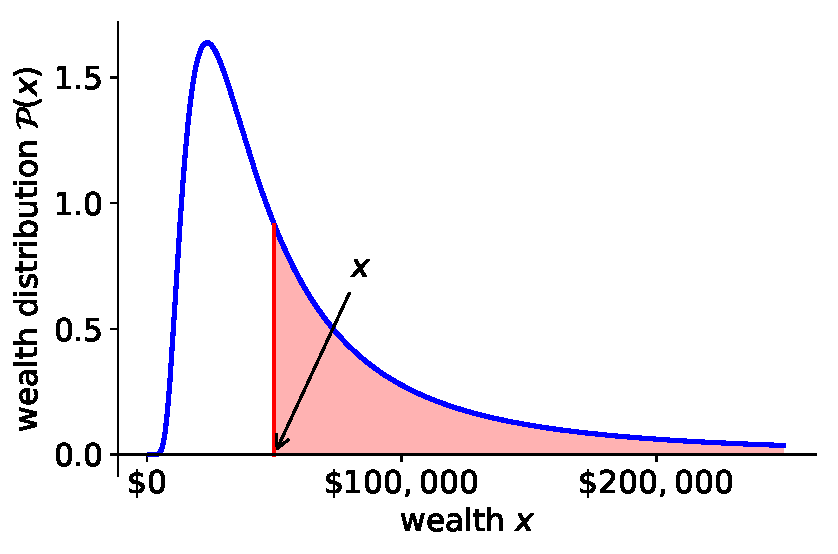
\includegraphics[width=.55\textwidth]{./chapter_people/figs/wealth_dist_def_2.pdf}}
\put(190,30){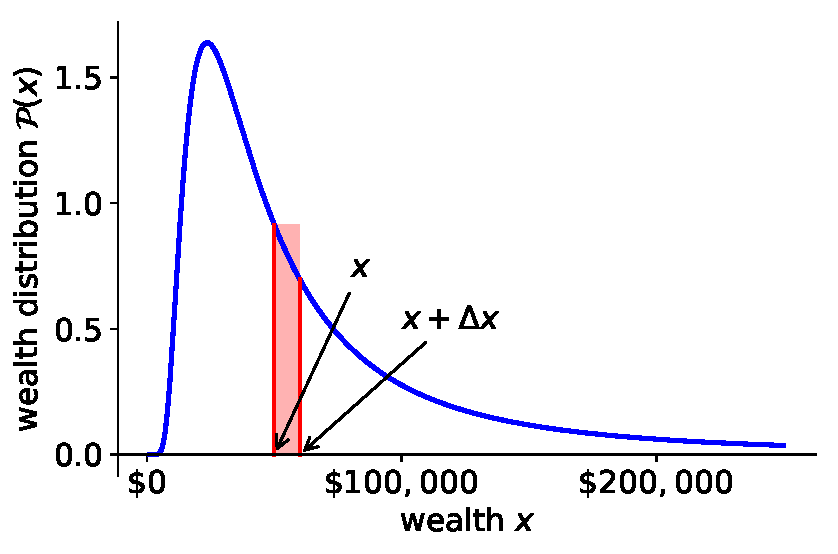
\includegraphics[width=.55\textwidth]{./chapter_people/figs/wealth_dist_def_1.pdf}}
\put(0,160){A)}
\put(190,160){B)}
\end{picture}
\caption{Example of a wealth distribution. A) The probability that a uniformly randomly selected person has wealth greater than $\x$ is the shaded area on the left. B) The number of people with wealth between $\x$ and $\x+\D\x$ is roughly $\N$ times the shaded area on the right.}
\flabel{wealth_dist_def}
\end{figure}

%%%%%%%%%%%%%%%%%%%%%%%%%%%%%%%%%%%%%%%

\subsection{Lognormal distribution}
\seclabel{Lognormal_wealth}
At a fixed time, $\t^\ast$, \GBM produces a random variable, $\x(\t^\ast)$, with a lognormal distribution whose parameters depend on $\t^\ast$. Recall that a lognormally distributed random variable is one whose logarithm is a normally distributed random variable. Suppose each individual's wealth follows \GBM,
\be
\gd\x=\x(\gmu \gd\t + \gsigma \gd\gW).
\elabel{GBM_SDE_ch6}
\ee
The solution of this \SDE, which we derived in \secref{Ito}, is
\be
\x(\t) = \x(0) \exp\left[\left(\gmu-\frac{\gsigma^2}{2}\right)\t + \gsigma \gW(\t)\right],
\ee
or, after taking logarithms,
\be
\ln\x(\t) = \ln\x(0) + \left(\gmu-\frac{\gsigma^2}{2}\right)\t + \gsigma \gW(\t).
\ee
From this we see that we will observe a lognormal distribution of wealth at each moment in time,
\be
\ln \x(\t) \sim  \mathcal{\N}\left(\ln \x(0) + \left(\gmu - \frac{\gsigma^2}{2}\right)\t, \gsigma^2 \t\right),
\elabel{lognormal}
\ee
as we showed in \eref{GBM_dist}. From now on we will assume the initial condition $\x(0)=1$ and, therefore, that $\ln \x(0)=0$ unless otherwise stated.

Note that the variance of $\ln \x(\t)$ increases linearly in time. We will develop an understanding of this shortly. As we will see, it indicates that any meaningful measure of inequality will grow over time in our simple model. To see what kind of a wealth distribution \eref{lognormal} is, it is worth spelling out the lognormal \PDFa:
\be
\PDF_x(\x)=\frac{1}{\x\sqrt{2\pi \gsigma^2t}}\exp\left(-\frac{[\ln \x-(\gmu-\frac{\gsigma^2}{2})\t]^2}{2\gsigma^2 \t} \right).
\elabel{PDFx}
\ee

This distribution is the subject of a wonderful book \cite{AitchisonBrown1957}, sadly out-of-print now but worth reading if you can find a copy. It will be useful to know some of its basic properties. Of particular importance is the expected wealth under this distribution. This is
\be
\ave{\x(\t)}=\exp(\gmu \t)
\elabel{exp_x}
\ee
or, equivalently, $\ln\ave{\x(\t)}=\gmu \t$.

We could confirm this result by calculating $\ave{\x(\t)}=\int_0^\infty s\PDF_\x(s) ds$, but that is laborious. Instead, we use a neat trick, courtesy of \cite[Chapter 4.2]{KloedenPlaten1992}, which will come in handy again in \secref{RGBM_moments}. The idea is to turn a stochastic differential equation for $\x$, like \eref{GBM_SDE_ch6}, into an ordinary differential equation for its $k^\text{th}$ moment, $\ave{\x^k}$. For the first moment, $k=1$, we do this simply by taking expectations of both sides of \eref{GBM_SDE_ch6}. The stochastic term vanishes to leave an ODE for the expected wealth, $\ave{\x}$:
\bea
\ave{\gd\x}&=&\ave{\x(\gmu \gd\t + \gsigma \gd\gW)}\\
d\ave{\x}&=&\ave{\x} \gmu \gd\t + \gsigma \overbrace{\ave{\gd\gW}}^{=0}\\
&=&\ave{\x} \gmu \gd\t.
\eea
This is a very simple first-order linear differential equation, whose solution with initial condition $\ave{\x(0)}=1$ is \eref{exp_x}.

For $\gmu>0$, the expected wealth grows exponentially over time, as do its median and variance:
\bea
\text{median}[\x(\t)] &=& \exp[(\gmu-\gsigma^2/2)\t]; \elabel{median_x} \\
\var[\x(\t)] &=& \exp(2\gmu \t)[\exp(\gsigma^2 \t)-1]. \elabel{var_x}
\eea

%%%%%%%%%%%%%%%%%%%%%%%%%%%%%%%%%%%%%%%

\subsection{Two growth rates}
\seclabel{two_rates}
We recap briefly one of our key ideas, covered in detail in \secref{Geometric_Brownian}, that the ensemble average of all possible trajectories of \GBM grows at a different (faster) rate from that achieved by a single trajectory almost surely in the long-time limit. Understanding this difference was the key to developing a coherent theory of individual decision-making. The difference is also crucial to understanding how wealth becomes distributed in a population of individuals whose wealths follow \eref{GBM_SDE_ch6}, and how we might measure the inequality in such a distribution.

Recall that the growth rate of the ensemble-average wealth is
\be
\gex = \frac{\D\ln\ave{\x}}{\Dt} = \gmu,
\ee
and that the time-average growth rate of wealth is
\be
\gt = \ave{\frac{\D\ln \x}{\Dt}} = \gmu-\frac{\gsigma^2}{2}.
\ee
Let us think about the structure of these growth rates.

We move on to our main goal: deriving the two growth rates of the economy. We found the solution for a single wealth trajectory under GBM and established that it grows exponentially at a normally distributed growth rate. We may now consider a population of such trajectories, such as might describe the wealths of people in an economy.

We reintroduce the person index $\gi$ and treat each individual wealth $\x_\gi(\t)$ as an independent trajectory generated by the stochastic process in \eref{GBM_SDE_ch6}. So our model population has incomes which evolve as
\be
\x_\gi(\t+\Dt) = \x_\gi(\t)\exp\left[\left(\gmu - \frac{\gsigma^2}{2}\right)\Dt + \gsigma \gW_\gi(\Dt)\right]\,,
\ee
for $\gi=1\dots N$. Note that we assume each person's income obeys GBM with the same drift and volatility parameters, $\gmu$ and $\gsigma$, but with different realisations of the noise in $\gW_\gi(\Dt)$.

Over the period $\Dt$, each person's wealth has a growth rate
\be
\g_\gi(\Dt) = \frac{\D\ln\x_\gi}{\Dt}\,.
\ee
These growth rates are $\N$ independent and identically distributed normal variates,
\be
\g_\gi(\Dt)  \sim \N\left(\gmu-\frac{\gsigma^2}{2}, \frac{\gsigma^2}{\Dt}\right)\,.
\elabel{gi}
\ee

\subsubsection{Democratic growth rate}
In the long time limit, $\Dt\to\infty$, the variance of the distribution in \eref{gi} tends to zero, meaning that the growth rates of all wealths converge to the same finite value. Eventually, therefore, this is the growth rate experienced by all individuals, so we denote it as
\be
\gt = \lim_{\Dt\to\infty}\left\{g_i(\Dt)\right\} = \gmu-\frac{\gsigma^2}{2}\,.
\elabel{gt}
\ee

As we know, the growth rate obtained in the long time limit is also obtained straightforwardly as the mean of the growth rates of wealth, the democratic growth rate, \ie
\be
\gt = \ave{\g(\Dt)} = \gmu-\frac{\gsigma^2}{2}\,.
\elabel{gt_equiv}
\ee
This is no coincidence. As we have discussed, changes in logarithmic income under GBM are stationary and independent. Crucially, this means they have the ergodic property. $\gt$ is one of the fundamental growth rates of the economy. It reflects the average rate at which a participant in the economy sees their income grow.

The ensemble average operator is linear, so we can write $\gt$ as
\be
\gt = \frac{\D\ave{\ln x}}{\Dt}\,.
\elabel{gt_general}
\ee

%\Eref{gt_general} demonstrates that to estimate $\gt$ the knowledge of individual growth rates is unnecessary. An immediate corollary is that $\gt$ is independent of income mobility. While $\gt$ measures the average growth rate experienced by individuals, and regardless of income mobility, $\gt$ only depends on the initial and terminal income distributions. Whether individuals earning higher incomes also experience higher growth rates than individuals with lower incomes, or the opposite, it does not change $\gt$ for specific initial and terminal income distributions. This has practical importance, since reliable panel data, required for estimating individual growth rates, are harder to obtain than data on the initial and terminal income distributions.

\subsubsection{Plutocratic growth rate}
An additional, and perhaps more familiar, growth rate of the economy is the growth rate of the ensemble average wealth. We can call this the plutocratic growth rate.

The evolution of the mean wealth, $\ave{\x(\t)}$, is found by taking the mean of both sides of \eref{GBM_SDE_ch6}, noting that $\ave{\gd\gW}=0$, to get
\be
\gd\ave{\x} = \ave{x}\gmu \gd\t\,.
\ee
The mean income grows exponentially,
%
\be
\ave{\x(\t+\Dt)}=\ave{\x(\t)}\exp(\gmu\Dt)\,,
\ee
%
and the growth rate of mean income is
%
\be
\gex = \frac{\D\ln\ave{\x}}{\Dt} = \gmu\,.
\ee
%

$\gex$ is another fundamental growth rates of the economy. It tells us how quickly the mean income and, multiplying by $N$, the aggregate income (or, in the terms of public discussion, the ``size of the economy'') are growing. It is an important statistic for central planners, who value being able to monitor and predict the total resources available to them for public spending.

Under GBM, $\gt$ is smaller than $\gex$ by the fluctuation dependent term $\gsigma^2/2$. More generally, in a large population, where individual incomes follow noisy multiplicative growth, the plutocratic growth rate is higher than the democratic growth rate experienced by individuals. Thus, using the the plutocratic growth rate as the principle measure of economic growth creates an impression that may be misleading.

%%%%%%%%%%%%%%%%%%%%%%%%%%%%%%%%%%%%%%%

\subsection{Measuring inequality}
\seclabel{Inequality_measure}
In the case of \GBM we have just seen how to 
compute the exact full wealth distribution, $\PDF_\x(\x)$. This is interesting but often we want only summary measures of the distribution. One summary measure of particular interest to economists is inequality. How much inequality is there in a distribution like \eref{lognormal}? And how does this quantity increase over time under \GBM, as we have suggested it does?

Clearly, to answer these questions, we must quantify ``inequality''. In this section, and also in \cite{AdamouPeters2016}, we develop a natural way of measuring it, which makes use of the two growth rates we identified for the non-ergodic process. We will see that a particular inequality measure, known to economists as Theil's second index \cite{Theil1967}, is a quantity which grows at the difference between the growth rates of average wealth (growing at the ensemble-average growth rate) and typical wealth (growing at the time-average growth rate) in the \GBM model. Thus, the difference between ensemble and time averages, the essence of ergodicity breaking, is the fundamental driver of the dynamics of inequality.

The two limits of inequality are easily identified. Minimum inequality means that everyone 
has the same wealth, so the wealth distribution is a Dirac delta function at the average wealth of the population, \ie the finite-ensemble average (\FEA). Thus, the minimally unequal distribution is
\be
\PDF_\x(\x)=\delta(\x-\ave{\x}_\N).
\ee
If we assume, for the moment, that individuals cannot have negative wealth, then maximum inequality means that one individual has all the wealth and everyone else has nothing.
The maximally unequal distribution is, therefore, composed of two Dirac delta peaks, one at zero wealth and one at the total wealth,
\be 
\PDF_\x(\x)=\frac{\N-1}{\N}\delta(\x-0)+\frac{1}{\N}\delta(\x-\N\ave{\x}_\N),
\ee
as shown in \fref{wealth_dist_extreme}.

\begin{figure}[h]
\begin{picture}(200,170)(20,30)
\put(0,30){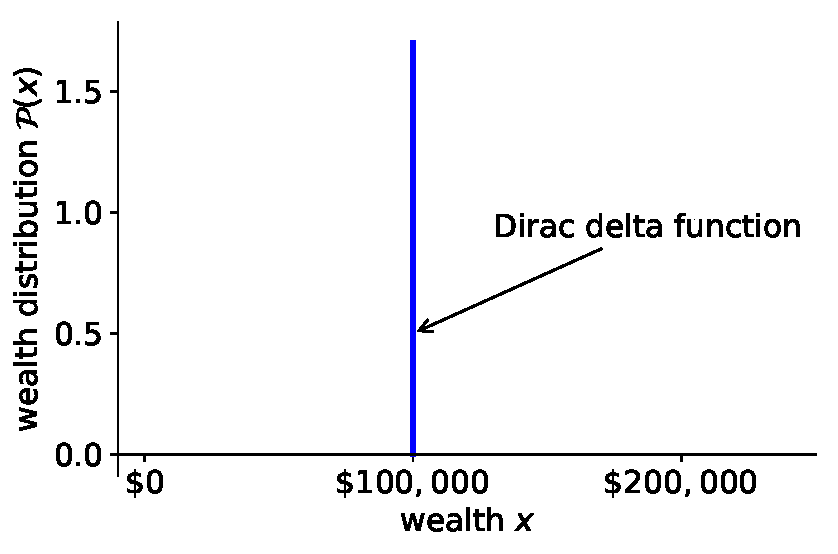
\includegraphics[width=.5\textwidth]{./chapter_people/figs/wealth_dist_equal.pdf}}
\put(190,30){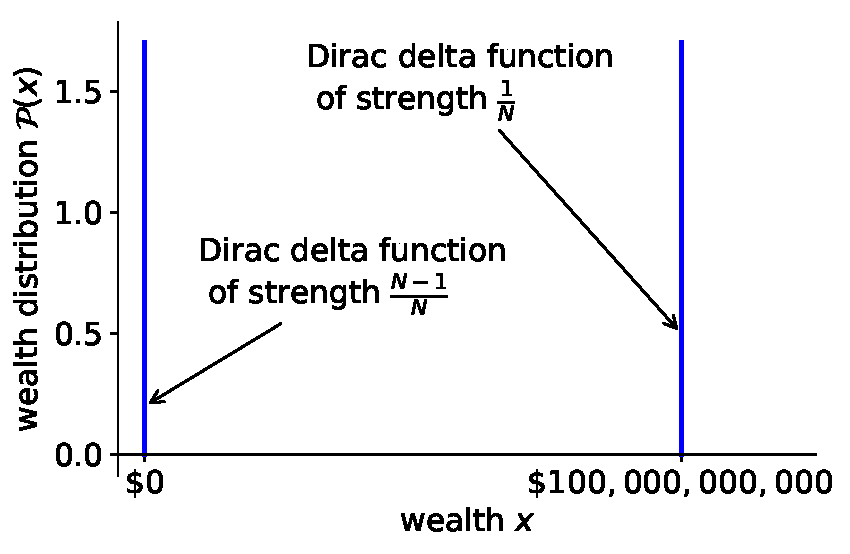
\includegraphics[width=.5\textwidth]{./chapter_people/figs/wealth_dist_unequal.pdf}}
\put(0,160){A)}
\put(190,160){B)}
\end{picture}
\caption{Extreme wealth distributions. A) The maximally equal distribution means that everyone owns the same amount (here \$100,000, as an example). B) The maximally unequal distribution (assuming no one has negative wealth) means that one person owns everything (here \$100 billion), and everyone else nothing.}
\flabel{wealth_dist_extreme}
\end{figure}

Quantifying inequality in any other distribution is reminiscent of the gamble 
problem. Recall that for gambles we wanted make statements of the type ``this gamble 
is more desirable than that gamble''. We did this by collapsing distributions, in this case of wealth changes in gambles, to scalars, which we could rank.
Depending on the question that was being asked, the appropriate way of collapsing the distribution and the resulting scalar can be different. (For example, the scalar relevant to an insurance company may not be relevant to an individual.)
In the case of inequality we also have a distribution -- the wealth distribution -- and we 
want to make statements of the type ``this distribution is more unequal than that 
distribution''. Again, this is done by collapsing the distribution to a scalar, and again 
many different choices of collapse and resulting scalar are possible. The Gini 
coefficient is a particularly well-known scalar of this type, the 80/20 ratio another. Indeed, there is a whole menagerie of inequality measures in economics.

In this context the expectation value is an important quantity. 
For instance, if everyone has the same wealth, then everyone will own the \FEA, $\x_\gi=\ave{\x}_\N$, which converges to the expectation value, $\ave{x}$, for large $\N$.
Furthermore, whatever the distribution of wealth, the total wealth is $\N\ave{\x}_\N$, whose relative difference from $\N\ave{\x}$ vanishes as $\N$ grows large.
The growth rate of the expectation value, $\gex$, thus tells us how fast the average wealth and the total wealth grow almost surely in a large population.

The time-average growth rate, $\gt$, on the other hand, tells us how fast an individual's wealth (indeed, \textit{every} individual's wealth) will grow almost surely in the $\t\to\infty$ limit.
So, over sufficiently long tome scales, $\gt$ will be the growth rate experienced by almost all members of a population.
If this typical growth rate is less than that of the expectation value of wealth, then there must be atypically wealthy individuals to account for the difference. This insight suggests the following measure of wealth inequality.

\definition{
Inequality, $\J$, is the quantity which grows at the difference between the growth rate of the ensemble average and the time-average growth rate,
\be
\frac{\gd \J}{\gd\t}=\gex-\gt.
\elabel{dJ}
\ee
\Eref{dJ} defines the dynamic of inequality, and inequality itself is found by 
integrating it over time:
\be
\J(\t)=\int_0^\t [\gex(s)-\gt(s)] \gd s
\elabel{J}
\ee
}

This definition may be used for dynamics other than \GBM, as we shall discuss in \secref{jensen}. Whatever the wealth dynamic, aggregate minus typical growth rates are informative of the dynamic of inequality. Within the \GBM framework we can write the difference in growth rates as 
\be
\frac{\gd \J}{\gd\t}=\frac{\gd \ln \ave{\x}}{\gd\t}-\frac{\gd \ave{\ln \x}}{\gd\t}
\elabel{J_dyn}
\ee
and integrate over time to get
\be
\J(\t)=\ln \ave{\x(\t)}-\ave{\ln \x(\t)}.
\elabel{J_x}
\ee
This quantity is known as the \MLD or Theil's second index of inequality \cite{Theil1967}. This is rather remarkable. Our general inequality measure, \eref{J}, evaluated for the specific case of \GBM, turns out to be a well-known measure of inequality that economists have identified independently, without considering the ergodicity problem. Merely by insisting on measuring inequality well, Theil used the \GBM model implicitly.\footnote{Like Kelly's ideas about gambling \cite{Kelly1956}, Theil's inequality measures emerged from information theory.}

Substituting the known values of the two growth rates into \eref{dJ} and integrating, we can evaluate the Theil inequality as a function of time:
\be
\J(\t)=\frac{\gsigma^2}{2} \t.
\elabel{J_t}
\ee
Thus we see that, in \GBM, our measure of inequality increases indefinitely.

%%%%%%%%%%%%%%%%%%%%%%%%%%%%%%%%%%%%%%%

\subsection{Wealth condensation}
\seclabel{condensation}
The lognormal distribution generated by \GBM broadens indefinitely, \eref{var_x}. Likewise, the inequality present in the distribution -- measured as the time-integrated difference between ensemble and time average growth rates -- grows without bound. A related property of \GBM is the evolution towards wealth condensation. Wealth condensation means that a single individual owns a non-zero fraction of the total wealth of the population in the $\N\to\infty$ limit, see \eg \cite{BouchaudMezard2000}. In the present case, an arbitrarily large share of the  total wealth will be owned by an arbitrarily small share of the population.

One simple way of seeing this is to calculate the fraction of the population whose wealths are less than the expected wealth, \ie $\x(\t)<\exp(\gmu \t)$. To do this, we define a new random variable, $z(\t)$, whose distribution is the standard normal:
\be
z(\t) \equiv \frac{\ln \x(\t) - (\gmu-\gsigma^2/2)\t}{\gsigma \t^{1/2}} \sim \mathcal{\N}(0,1).
\ee
We want to know the mass of the distribution with $\ln \x(\t)<\gmu \t$. This is equivalent to $z<\gsigma \t^{1/2}/2$, so the fraction below the expected wealth is
\be
\gPhi\left(\frac{\gsigma \t^{1/2}}{2}\right),
\ee
where $\gPhi$ is the \CDF of the standard normal distribution. This increases over time, tending to one as $\t\to\infty$. \AA{Plot this?}

%%%%%%%%%%%%%%%%%%%%%%%%%%%%%%%%%%%%%%%

\subsection{Rescaled wealth}
\seclabel{rescaled}
Economists have arrived at many inequality measures, and have drawn up a list of conditions that particularly useful measures of inequality satisfy. Such measures are called ``relative measures'' \cite[Appendix 4]{Sen1997} and $\J$ is one of them.

One of the conditions is that inequality measures should not change when $\x$ is divided by the same factor for everyone. Since we are primarily interested in inequality in this section, we can remove absolute wealth levels from the analysis and study an object called the rescaled wealth.

\definition{
The rescaled wealth of an individual, 
\be
\gw_\gi(\t) = \frac{\x(\t)}{\ave{\x(\t)}_\N},
\elabel{rescaled}
\ee
is the fraction of the average wealth of the population (\ie the \FEA) owned by that individual.}

This quantity is useful because its numerical value does not 
depend on the currency used: it is a dimensionless number. 
Thus if my rescaled wealth is $\gw_\gi(\t) = 1/2$, it means that my wealth is half the 
average wealth, irrespective of whether I measure it in Kazakhstani Tenge 
or in Swiss Francs. The \FEA of rescaled wealth is easily calculated:
\be
\ave{\gw_\gi(\t)}_\N = \ave{\frac{\x(\t)}{\ave{\x(\t)}_\N}}_\N = 1.
\ee

If the population size, $\N$, is large enough, then we might expect the \FEA wealth, $\ave{\x(\t)}_\N$, to be close to the ensemble average, $\ave{\x(\t)}$, which is simply its $\N\to\infty$ limit. We will discuss more carefully when this approximation holds in the \GBM model in \secref{finite_populations}. Let's assume for now that it does. The rescaled wealth is then well approximated as
\be
\gw_\gi(\t) = \frac{\x_\gi(\t)}{\ave{\x(\t)}} = \x_\gi(\t)\exp(-\gmu \t).
\ee

Now that we have an expression for $\gw$ in terms of $\x$ and $\t$, we can derive the dynamic for rescaled wealth using \Ito's formula (just as we did to find the wealth dynamic for a general utility function in \secref{from_ergo}). We start with
\bea
\gd \gw &=& \frac{\partial \gw}{\partial \t}\gd\t + \frac{\partial \gw}{\partial \x}\gd\x + \frac{1}{2} \frac{\partial^2 \gw}{\partial \x^2} \gd\x^2 \\
&=& -\gmu \gw\gd\t + \frac{\gw}{\x}\gd\x \elabel{ysde},
\eea
and then substitute \eref{GBM_SDE_ch6} for $\gd\x$ to get
\be
\gd \gw = \gw \gsigma \gd\gW.
\elabel{GBM_y}
\ee
So $\gw(\t)$ follows a very simple \GBM with zero drift and volatility $\gsigma$. This means that rescaled wealth, like wealth, has an ever-broadening lognormal distribution:
\be
\ln \gw(\t) \sim \mathcal{\N}\left(-\frac{\gsigma^2}{2}\t, \gsigma^2 \t\right).
\elabel{lognormal_y}
\ee

Finally, noting that $\ave{\ln \gw}=\ave{\ln \x}-\ln\ave{\x}$ gives us a simple expression for our inequality measure in \eref{J_x} in terms of the rescaled wealth:
\be
\J(\t)=-\ave{\ln \gw}.
\ee

%%%%%%%%%%%%%%%%%%%%%%%%%%%%%%%%%%%%%%%

\subsection{Jensen's inequality and $\gv$-normal distributions}
\seclabel{jensen}
So far we have confined our analysis to \GBM, where wealths follow the dynamic specified by \eref{GBM_SDE_ch6}. However, as we discussed in the context of gambles, other wealth dynamics are possible. In particular, we explored the dynamics corresponding to ergodicity transformations that execute a \BM with drift as in \eref{dv_gen}:
\be
\gd\gv = a_\gv \gd\t + b_\gv \gd\gW.
\ee
Under this dynamic, $\gv$ is normally distributed,
\be
\gv(\x(\t)) \sim \mathcal{\N}\left(a_\gv\t, {b_\gv}^2 \t\right),
\ee
and we can say that wealth has a ``$\gv$-normal'' distribution. For \GBM, the ergodicity transformation, as we know, is $\gv(\x)=\ln \x$, and $\gv$-normal becomes lognormal.

Replacing the logarithm in \eref{J_x} by the general ergodicity transformation gives a general expression for our wealth inequality measure,
\be
\J_\gv(\t)=\gv(\ave{\x(\t)}) - \ave{\gv(\x(\t))}.
\elabel{J_u}
\ee
It's not easy to write a general expression for $\J_\gv(\t)$ in only $\t$ and the model parameters $a_\gv$ and $b_\gv$, because it would involve the solution of the general wealth dynamic in \eref{dx}. \AA{Is this true?} However, we can still say something about how inequality evolves. Let's see what happens if we start with perfect equality, $\x_\gi(0)=\x_0$ with $\x_0$ fixed, and then let wealths evolve a little to $\x(\D \t)=\x_0+\D \x$, where $\D \x$ is a random wealth increment generated by the wealth dynamic. The change in inequality would be
\be
\D \J_\gv = \gv(\ave{\x_0+\D \x}) - \ave{\gv(\x_0+\D \x)},
\ee
since $\gv(\ave{\x_0})=\ave{\gv(\x_0)}=\gv(\x_0)$.

We can now appeal to Jensen's inequality: if $\gv$ is a concave function, like the logarithm, then $\D \J_\gv \geq 0$; while if $\gv$ is convex, like the curious exponential in \eref{test_dyn_u}, then $\D \J_\gv \leq 0$. The only cases for which $\D \J_\gv=0$ are if $\D \x$ is non-random or if $\gv$ is linear. Thus, it is both randomness and the nonlinearity of the ergodicity transformation -- or ``utility function'' if we make that equivalence -- that creates a difference in growth rates and generates inequality.

%%%%%%%%%%%%%%%%%%%%%%%%%%%%%%%%%%%%%%%

\subsection{Power-law resemblance}
\seclabel{power_law}
It is an established empirical observation \cite{Newman2005} that the upper tails of 
real wealth distributions look more like a power-law than a lognormal. Our trivial model does not
strictly reproduce this feature, but it is instructive to compare the lognormal distribution
to a power-law distribution. A power-law \PDFa has the asymptotic form 
\be
\PDF_\x(\x)= \x^{-\alpha},
\elabel{power_law}
\ee
for large arguments $\x$. This implies that the logarithm of the \PDFa is proportional 
to the logarithm of its argument, $\ln \PDF_\x(\x) = -\alpha \ln \x$. Plotting
one against the other will yield a straight line, the slope being the exponent $-\alpha$. 

Determining whether an empirical observation is consistent with such behaviour 
is difficult because the behaviour to be observed is in the tail (large $\x$) where data are,
by definition, sparse. A quick-and-dirty way of checking for possible power-law 
behaviour is to plot an empirical \PDFa against its argument on log-log scales, 
look for a straight line, and measure the slope. However, plotting any distribution on any 
type of scales results in some line. It may not be a straight line but it will have some slope 
everywhere. For a known distribution (power-law or not) we can interpret this slope 
as a local apparent power-law exponent. 

What is the local apparent power-law exponent of a lognormal wealth distribution near the 
expectation value $\ave{\x}=\exp(\gmu \t)$, \ie in the upper tail where approximate power-law behaviour
has been observed empirically? The logarithm of \eref{PDFx} is
\bea
\ln \PDF(\x) =& -\ln\left(\x\sqrt{2\pi \gsigma^2t}\right) -\frac{[\ln \x-(\gmu-\frac{\gsigma^2}{2})\t]^2}{2\gsigma^2 \t}\\
=& -\ln \x -\frac{\ln (2\pi \gsigma^2t)}{2} - \frac{(\ln \x)^2-2(\gmu-\frac{\gsigma^2}{2})\t \ln \x+(\gmu-\frac{\gsigma^2}{2})^2t^2}{2\gsigma^2 \t}.
\eea
Collecting terms in powers of $\ln \x$ we find
\be
\ln \PDF(\x)=-\frac{(\ln \x)^2}{2\gsigma^2 \t}  + \left(\frac{\gmu}{\gsigma^2}-\frac{3}{2}\right)\ln \x - \frac{\ln(2 \pi\gsigma^2 \t)}{2}-\frac{(\gmu-\frac{\gsigma^2}{2})^2t}{2\gsigma^2}
\ee
with local slope, \ie apparent exponent,
\be
\frac{\gd\ln \PDF(\x)}{\gd \ln \x} = - \frac{\ln \x}{\gsigma^2 \t}  + \frac{\gmu}{\gsigma^2} - \frac{3}{2}.
\ee
Near $\ave{\x}$, $\ln \x \sim \gmu \t$ so that the first two terms cancel approximately. Here the distribution will resemble a power-law with exponent $-3/2$ when plotted on doubly logarithmic scales. (The distribution will also look like a power law where the first term is much smaller than the others, \eg where $\ln \x \ll \gsigma^2 \t$.) We don't believe that empirically observed power laws are merely a manifestation of this mathematical feature. Important real-world  mechanisms that broaden real wealth distributions, \ie concentrate wealth, are missing from the null model, and we will see that including interactions among individuals produces a proper power-law tail in the distribution whose exponent is closer to observations than $-3/2$. However, it is interesting that the trivial model of \GBM reproduces so many qualitative features of empirical observations. 

%%%%%%%%%%%%%%%%%%%%%%%%%%%%%%%%%%%%%%%

\section{Finite populations}
\seclabel{finite_populations}
So far we have considered the properties of the random variable, $\x(\t)$, generated by \GBM at a fixed time, $\t$. Most of the mathematical objects we have discussed are, strictly speaking, relevant only in the limit $\N\to\infty$, where $\N$ is the number of realisations of this random variable. For example, the expected wealth, $\ave{\x(\t)}$, is the $\N\to\infty$ limit of
\be
\ave{\x(\t)}_\N \equiv \frac{1}{\N}\sum_{i=1}^\N \x_\gi(\t),
\elabel{FEA}
\ee
which we introduced in \secref{ensemble_average} as the finite-ensemble average (\FEA).

In reality, human populations can be very large, say $\N\sim10^7$ for a nation state, but they are most certainly finite. Therefore, we need to be diligent and ask under what conditions the results we have derived in the large-$N$ limit are valid for finite populations. In particular, we will focus on the \FEA wealth under \GBM. For what values of $\gmu$, $\gsigma$, $\t$, and $\N$ is this well approximated by the expectation value? And when it is not, what does it resemble?

\subsection{Sums of lognormals}
\seclabel{sketch}
In \cite{PetersKlein2013} we studied the \FEA, \eref{FEA}, of trajectories, $\x_\gi(\t)$, of \GBM. We know that at a given time $\t^\ast$, $\x(\t^\ast)$ is a random variable with a lognormal distribution. Therefore, the object of our interest is, essentially, a sum of lognormal variates. Here we sketch out some simple arguments, which we presented in \cite{PetersAdamou2018b}, about how this object depends on $\N$ and $\t$.

Considering the two growth rates in \secref{two_rates}, we anticipate a tension between two limiting scenarios:
\begin{itemize}
\item for large $\N$, the \FEA should resemble the expectation value, $\exp(\gmu \t)$;
\item for large $\t$, all trajectories in the finite-ensemble, and therefore the \FEA itself, should grow like $\exp[(\gmu-\gsigma^2/2)\t]$.
\end{itemize}
The first scenario, when a \FEA resembles the corresponding expectation value, is known in statistical physics as ``self-averaging.'' A simple strategy for estimating when this occurs is to look at the relative variance of the \FEA,
\be
R \equiv \frac{\var[\ave{\x(\t)}_\N]}{\ave{\ave{\x(\t)}_\N}^2}.
\elabel{rel_var}
\ee
To be explicit, the $\text{var}[\cdot]$ and $\ave{\cdot}$ operators, without subscript $\N$, refer to the mean and variance over all possible realisations of the random variables enclosed, which in \eref{rel_var} are \FEAs. The \FEAs themselves, taken over finite samples of wealth realisations, are denoted by the $\ave{\cdot}_\N$ operator, with subscript $N$ indicating the sample size.

\Eref{rel_var} simplifies to
\be
R = \frac{\frac{1}{\N}\var[\x(\t)]}{\ave{\x(\t)}^2},
\ee
into which we insert \eref{exp_x} and \eref{var_x} to get an expression in terms of the \GBM model parameters:
\be
R = \frac{\exp(\gsigma^2 \t)-1}{\N}.
\elabel{rel_var_N}
\ee
If $R \ll 1$, then the \FEA will likely be close to its own expectation value, which is equal to the expectation value of the \GBM. Therefore, under our convention that $x(0)=1$, we have
\be
\ave{\x(\t)}_\N\approx\ave{\x(\t)} = \exp(\gmu\t)
\elabel{self_ave}
\ee
when
\be
\t < \frac{\ln \N}{\gsigma^2}.
\elabel{short_t}
\ee
This hand-waving argument tells us roughly when the self-averaging regime holds: yes, for large enough samples, as we anticipated above, but equivalently for short enough time or low enough volatility. A more careful estimate of the critical time, shown later in in \eref{t_c}, is a factor of 2 larger, but its scaling with sample size and volatility is identical.

Self-averaging stops when even the ``luckiest'' trajectory is no longer close to the expectation value $\exp(\gmu \t)$. This is guaranteed to happen eventually because the probability for a trajectory to reach $\exp(\gmu \t)$ decreases towards zero as $\t$ grows, as we saw in \secref{condensation}. Naturally, this takes longer for larger samples, which have more chances to contain a lucky trajectory.

For $\t>\ln \N/\gsigma^2$, the growth rate of the \FEA transitions from $\gmu$ to its $\t\to\infty$ limit of $\gmu-\gsigma^2/2$. For finite $\N$ and $\t$, we can estimate the value of the \FEA by thinking about what dominates the average. For early times in the process, all trajectories are close together and none dominate the \FEA. However, as time goes by the distribution broadens exponentially. Since each trajectory contributes with the same $1/\N$ weight to the \FEA, we speculate that after some time the \FEA will be dominated by the maximum in the sample, \ie
\be
\ave{\x(\t)}_\N \approx \frac{1}{\N}\max_{\gi=1}^\N \{\x_\gi(\t)\}.
\elabel{max_N}
\ee

These features are consistent with the numerical simulations in \fref{trajectories}, which we suggest as an exercise. With our intuition thus corroborated, it is worth the effort to say something more about \eref{max_N} using extreme value theory. The maximum of a sample of $\N$ iid standard normal variates, $\xi_\gi\sim\mN(0,1)$ for $\gi=1\dots\N$, is distributed around a mean which scales like
\be
\ave{\max_{\gi=1}^\N \{\xi_\gi\}} \approx \sqrt{2\ln\N}
\ee
to leading order in the $\N\to\infty$ limit.\footnote{A fuller approximation is
\be
\ave{\max_{\gi=1}^\N \{\xi_\gi\}} = \sqrt{\ln\left(\frac{\N^2}{2\pi\ln\left(\N^2/2\pi\right)}\right)}\left[1+\frac{\gamma}{\ln\N}+o\left(\frac{1}{\ln\N}\right)\right],
\ee
where $\gamma=0.57721\dots$ is the Euler-Mascheroni constant.} Since
\be
\x_\gi(\t) = \exp\left[\left(\gmu-\frac{\gsigma^2}{2}\right)\t + \gsigma\t^{1/2}\xi_\gi\right]
\ee
increases monotonically with $\xi_\gi$, the largest $\x_\gi(\t)$ is that corresponding to the largest $\xi_\gi$ in the sample. Therefore, for large samples we anticipate that
\be
\ave{\x(\t)}_\N \approx \frac{1}{N} \exp\left[\left(\gmu-\frac{\gsigma^2}{2}\right)\t + \sqrt{2\ln\N} \gsigma\t^{1/2}\right]
\elabel{long_t_EVT}
\ee
after self-averaging breaks down, $\t>\ln\N/\gsigma^2$. Note that the first term in the exponent dominates as $\t\to\infty$, so the growth rate tends to that of a single trajectory, $\gmu-\gsigma^2/2$, as we have argued it must.

\begin{figure}[h]
\centering
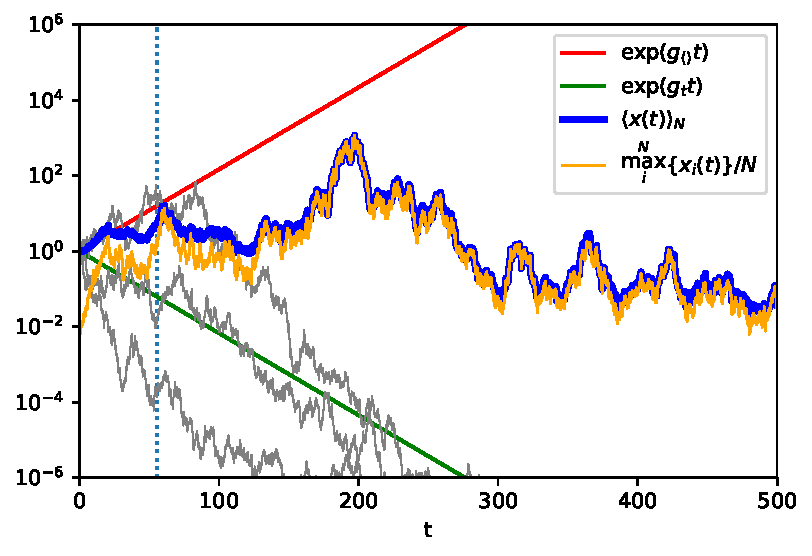
\includegraphics[height=9.3cm]{./chapter_people/figs/trajectories.pdf}
\caption{\FEA and maximum in a finite ensemble of size $\N=256$. {\bf \underline{Red line:}} expectation value $\ave{\x(\t)}$. 
{\bf \underline{Green line:}} exponential growth at the time-average growth rate. In the $\t\to\infty$ limit all trajectories grow at this rate. 
{\bf \underline{Yellow line:}} contribution of the maximum value of any trajectory at time $\t$ to the \FEA.  
{\bf \underline{Blue line:}} \FEA $\ave{\x(\t)}_\N$.
{\bf \underline{Vertical line:}} Crossover -- for $\t>\tc=\frac{2\ln \N}{\gsigma^2}$ the maximum begins to dominate the \FEA (the yellow line approaches the blue line).
{\bf \underline{Grey lines:}} randomly chosen trajectories -- any typical trajectory soon grows at the time-average growth rate.  
{\bf \underline{Parameters:}} $\N=256$, $\gmu=0.05$, $\gsigma=\sqrt{0.2}$.}
\flabel{trajectories}
\end{figure}

We now have two approximations, \eref{self_ave} and \eref{long_t_EVT}, for the \FEA in and out of the self-averaging regime. We can express these as approximations to the growth rate, $\g_\N(\t)$, of a \FEA of size $\N$ after time $\t$:
\bea
\g_\N(\t) &=&  \frac{\ln\ave{\x(\t)}_N - \ln\ave{\x(0)}_N}{\t-0} \\
&\approx&
\begin{cases}
\gmu, & 0 < \t < \frac{\ln\N}{\gsigma^2}; \\
\gmu - \frac{\gsigma^2}{2} - \frac{\ln\N}{\t} + \frac{\sqrt{2\ln\N}\gsigma}{\t^{1/2}}, & \t > \frac{\ln\N}{\gsigma^2}.
\end{cases}
\elabel{g_N_EVT}
\eea

\subsection{The random energy model}
\seclabel{REM}
In \cite{PetersKlein2013} we analysed \FEAs of \GBM analytically and numerically. Using \eref{GBM_sol} with $x(0)=1$, the \FEA can be written as
\be
\ave{\x(\t)}_\N=\frac{1}{\N} \sum_{\gi=1}^\N \exp\left[ \left(\gmu-\frac{\gsigma^2}{2}\right) \t + \gsigma \gW_\gi(\t) \right],
\elabel{FEA}
\ee
where the $\gW_\gi(\t)$ are independent trajectories of the Wiener process. Taking the deterministic part out of the sum, we can write
\be
\ave{\x(\t)}_\N = \frac{1}{\N} \exp\left[ \left(\gmu-\frac{\gsigma^2}{2}\right) \t \right] \sum_{\gi=1}^\N \exp\left(\gsigma \t^{1/2} \xi_\gi\right),
\elabel{FEA_2}
\ee
where the $\xi_\gi$ are independent standard normal variates. All of the uncertainty in the value of the \FEA is now contained in the sum of lognormal variates, which we denote by 
\be
Z(\N,\t) = \sum_{\gi=1}^\N \exp\left(\gsigma \t^{1/2} \xi_\gi\right),
\elabel{FEA_Z}
\ee
such that $\ave{\x}_\N = \left(1/N\right) \exp\left[ \left(\gmu-\gsigma^2/2\right) \t \right] Z(\N,t)$.

Since the publication of \cite{PetersKlein2013} we learned, thanks to discussions with J.-P.~Bouchaud, that $Z(\N,\t)$, the sum of lognormal random variates, has been of interest to the mathematical physics community since the 1980s. The reason for this is B.~Derrida's random energy model \cite{Derrida1980,Derrida1981}, which we will describe here.

Imagine a physical system with $K$ spins, whose $\N=2^K$ energy levels are normally distributed random energies, $E\xi_\gi$, with standard deviation, $E$. This is a simple model of a disordered system, such as a spin glass, the idea being that the system is so complicated that we ``give up'' trying to model it deterministically and instead model its energy levels as realisations of a random variable. (If this doesn't mean much to you, don't worry. All we really care about is that there are $\N$ random variables, which happen to be energies.)

The partition function is a sum of lognormal variates,
\be
\mZ(\N,T) = \sum_{\gi=1}^{\N} \exp\left(\frac{E\xi_\gi}{T}\right),
\elabel{Z}
\ee
where $T$ is the temperature and the energy parameter scales like $E \propto K^{1/2}$ to ensure an extensive thermodynamic limit \cite[p.~79]{Derrida1980}. The Helmholtz free energy is
\be
\mF = -T\ln\mZ,
\elabel{F}
\ee
and Derrida studied the expectation value of the free energy,
\be
\ave{\mF} = -T\ave{\ln\mZ},
\ee
which is an ensemble average over all possible realisations of the partition function, \ie over all possible samples of $\N$ lognormal variates. He found a critical temperature, $T_c$, and expressions for $\ave{\mF}$ valid in the high ($T>T_c$) and low ($T<T_c$) temperature regimes of the model.

These expressions for $\ave{\mF}$ are extremely useful for us, although we won't present their derivation here.\footnote{If you are interested in the derivation, Derrida's original papers \cite{Derrida1980,Derrida1981} are more penetrable than many in statistical physics, and the random energy model is taught in many university statistical physics courses.} $\mZ(\N,T)$, is the same type of mathematical object as $Z(\N,\t)$ in \eref{FEA_Z}, namely a sum of lognormal variates. Therefore, Derrida's results about $\mZ$ provide analogous results about $Z$. All we need to do is map from the parameters of the random energy model to those of \GBM, a slightly tedious algebraic exercise which results in
\be
\ave{\ln Z(\N,\t)} =
\begin{cases}
\ln\N + \frac{\gsigma^2 \t}{2}, & 0 < \t < \tc, \\
\sqrt{2 \ln\N} \gsigma \t^{1/2}, & \t > \tc,
\end{cases}
\elabel{ln_Z_exp}
\ee
where
\be
\tc = \frac{2\ln\N}{\gsigma^2}.
\elabel{t_c}
\ee
$\tc$ the critical time scale, delineating the short-time ($\t<\tc$) and long-time ($\t>\tc$) regimes of our model, corresponding respectively to the high-temperature ($T>T_c$) and low-temperature ($T<T_c$) phases in Derrida's model.

Note that $\tc$ in \eref{t_c} scales with $\N$ and $\gsigma$ identically to the self-averaging time we found in \secref{sketch}, using only the simple argument that the relative variance of the \FEA be small. The only difference is a factor of 2. It is pleasing that our intuition there was consistent with a careful analysis from statistical physics.

Armed with \eref{ln_Z_exp}, what can we say about the properties of the \FEA in \GBM? Let's write down growth rate experienced by a \FEA of size $\N$ after time $\t$: 
\bea
\g_\N(\t) &=& \frac{1}{\t} \left[ \ln \ave{\x(\t)}_\N - \ln \x(0) \right] \\
&=& \frac{1}{\t} \ln \left( \frac{1}{\N} \exp\left[\left(\gmu - \frac{\gsigma^2}{2}\right) \t \right] Z(\N,\t) \right) \\
&=& \gmu - \frac{\gsigma^2}{2} - \frac{\ln\N}{\t} + \frac{\ln Z}{\t}.
\elabel{g_N}
\eea
This is a random variable, with all the randomness contained in $\ln Z$ in the final term. We know the expectation values taken by $\ln Z$ in the short- and long-time regimes, \eref{ln_Z_exp}. Therefore, taking the expectation of \eref{g_N} and substituting for $\ave{\ln Z}$ gives us expectation values of the growth rate of the \FEA:
\be
\ave{\g_\N(\t)} =
\begin{cases}
\gmu, & 0 < \t < \tc; \\
\gmu - \frac{\gsigma^2}{2} - \frac{\ln\N}{\t} + \frac{\sqrt{2\ln\N}\gsigma}{\t^{1/2}}, & \t > \tc.
\end{cases}
\elabel{g_N_exp}
\ee
Perhaps surprisingly, these expected growth rates match perfectly the approximate growth rates presented in \eref{g_N_EVT}, which we found by considering what dominates the \FEA in the two regimes (and by applying a small dose of extreme value theory in the long-time regime).